
\documentclass{article}
\usepackage{circuitikz}
\usepackage{graphicx}
\begin{document}
\begin{figure}[!ht]
\centering
\resizebox{0.7\textwidth}{!}{
\begin{circuitikz}
\tikzstyle{every node}=[font=\LARGE]
\draw [ fill={rgb,255:red,240; green,240; blue,240} ] (10,12) rectangle  node {\LARGE Vorverstärker} (15,10.75);
\draw [line width=1pt, short] (12.5,10.75) -- (12.5,3.25);
\draw [line width=1pt, ->, >=Stealth] (12.5,5.75) -- (8.5,5.75);
\draw [line width=1pt, ->, >=Stealth] (12.5,3.25) -- (5,3.25);
\draw [ fill={rgb,255:red,240; green,240; blue,240} , line width=1pt ] (-1.25,4.5) rectangle  node {\LARGE Computer/Elektronik} (5,1.75);


\draw [line width=1pt, short] (11.25,4) -- (11.25,5);
\draw [line width=1pt, ->, >=Stealth] (11.25,5) -- (8.75,5);
\draw [ fill={rgb,255:red,240; green,240; blue,240} , line width=1pt ] (5.75,5.125) -- (5.75,5.125) -- (5.75,5.125) -- (5.75,5.125) -- cycle;
\draw [ fill={rgb,255:red,240; green,240; blue,240} , line width=1pt ] (7.25,5.25) rectangle (7.25,5.25);
\draw [ fill={rgb,255:red,240; green,240; blue,240} , line width=1pt ] (4.75,6) rectangle (4.75,6);
\draw [ fill={rgb,255:red,240; green,240; blue,240} , line width=1pt ] (5.75,5.5) rectangle (5.75,5.5);
\draw [ fill={rgb,255:red,240; green,240; blue,240} , line width=1pt ] (5.75,5.5) rectangle (5.75,5.5);
\draw [ fill={rgb,255:red,240; green,240; blue,240} , line width=1pt ] (2.5,3.5) rectangle (2.5,3.5);
\draw [ fill={rgb,255:red,240; green,240; blue,240} , line width=1pt ] (6.25,5.75) rectangle (6.25,5.75);
\draw [ fill={rgb,255:red,240; green,240; blue,240} , line width=1pt ] (6,5.5) rectangle (6,5.5);
\draw [ fill={rgb,255:red,240; green,240; blue,240} , line width=1pt ] (6,5.5) rectangle (6,5.5);
\draw [ line width=1pt](7.25,5.75) to[short, -o] (7.25,5.75) ;
\draw [ line width=1pt](7.25,5.75) to[short, -o] (7.25,5.75) ;
\draw [ line width=1pt](6.75,5.25) to[short, -o] (6.75,5.25) ;
\draw [ fill={rgb,255:red,240; green,240; blue,240} , line width=1pt , rotate around={180:(6.75,5.25)}] (4.75,6) -- (8.25,6) -- (8.75,4.5) -- (5.25,4.5) -- cycle;
\node [font=\LARGE] at (6.75,5.25) {Regelkreis}; 
\draw [line width=1pt, short] (1.25,4.5) -- (1.25,9.5);
\draw [ fill={rgb,255:red,240; green,240; blue,240} , line width=1pt ] (1.25,5.75) circle (0cm);
\draw [ fill={rgb,255:red,0; green,0; blue,0} , line width=1pt ] (1.25,5.75) circle (0.25cm);
\draw [line width=1pt, short] (1.25,5.75) -- (4.75,5.75);
\draw [line width=1pt, short] (6.25,7.5) -- (6.25,7.5);
\draw [ fill={rgb,255:red,240; green,240; blue,240} , line width=1pt ] (-1.25,12) rectangle  node {\huge Z-Piezokristall} (3.75,9.5);
\draw [ fill={rgb,255:red,240; green,240; blue,240} , line width=1pt ] (1.25,8.5) rectangle (1.25,8.5);
\draw [ fill={rgb,255:red,240; green,240; blue,240} , line width=1pt ] (-1.25,12) rectangle (-3.75,17);
\node [font=\LARGE, rotate around={90:(0,0)}] at (-2.5,14.5) {X/Y-Piezokristall};
\draw [ fill={rgb,255:red,240; green,240; blue,240} , line width=1pt , rotate around={90:(-2.75, 14.5)}] (-2.75,14.5) rectangle (-2.75,14.5);
\draw [ fill={rgb,255:red,240; green,240; blue,240} , line width=1pt , rotate around={90:(-1.75, 17)}] (-1.75,17) rectangle (-1.75,17);
\draw [ fill={rgb,255:red,240; green,240; blue,240} , line width=1pt , rotate around={90:(-3, 16)}] (-3,16) rectangle (-3,16);
\draw [ fill={rgb,255:red,240; green,240; blue,240} , line width=1pt , rotate around={90:(-3, 14.75)}] (-3,14.75) rectangle (-3,14.75);
\draw [ fill={rgb,255:red,240; green,240; blue,240} , line width=1pt ] (4.75,19.25) rectangle (4.75,19.25);
\draw [ fill={rgb,255:red,243; green,205; blue,205} , line width=1pt ] (3.75,12) rectangle  node {\huge Tunnelspitze} (-1.25,17.75);
\draw [line width=1pt, short] (-1.25,17.75) -- (1.25,20.75);
\draw [line width=1pt, short] (3.75,17.75) -- (1.25,20.75);
\foreach \x in {0,...,3}{
  \draw [ line width=1pt] (-3.75+\x*2.5,22) -- ++(1.25,2.45) -- ++ (1.25, -2.45);
}
\draw [line width=1pt, short] (-3.75,22) -- (-3.75,25.75);
\draw [line width=1pt, short] (5.5,23.5) -- (5.5,23.5);
\draw [line width=1pt, short] (6.25,25.75) -- (6.25,22);
\draw [line width=1pt, short] (-3.75,25.75) -- (6.25,25.75);
\node [font=\huge] at (1.25,25) {Probe};
\draw [line width=1pt, short] (3.75,14.5) -- (12.5,14.5);
\draw [line width=1pt, ->, >=Stealth] (12.5,14.5) -- (12.5,12);
\node [font=\huge] at (8.25,15) {Tunnelstromsignal};
\node [font=\LARGE, rotate around={90:(0,0)}] at (0.5,7.5) {Z-Steuerung};
\draw [line width=1pt, short] (-6.25,14.5) -- (-3.75,14.5);
\draw [line width=1pt, short] (-6.25,14.5) -- (-6.25,3.25);
\draw [line width=1pt, short] (-6.25,3.25) -- (-1.25,3.25);
\node [font=\LARGE, rotate around={90:(0,0)}] at (-6.75,8.5) {X-Y-Rasterbewegung};
\node [font=\LARGE, rotate around={90:(0,0)}] at (-9.5,10.5) {};
\draw (8.5,24) to[battery1,l=$U$] (8.5,17.5);
\draw [line width=1pt, short] (5.25,13.25) -- (3.75,13.25);
\draw [line width=1pt, short] (5.25,15.25) -- (5.25,17.5);
\draw [line width=1pt, short] (5.25,13.75) .. controls (4.5,13.75) and (4.5,15.25) .. (5.25,15.25);
\draw [line width=1pt, ->, >=Stealth] (1.75,1.75) -- (1.75,0.25);
\draw [ fill={rgb,255:red,240; green,240; blue,240} , line width=1pt , rotate around={90:(-1.25, -0.5)}] (-1.25,-0.5) rectangle (-1.25,-0.5);
\draw [ fill={rgb,255:red,240; green,240; blue,240} , line width=1pt ] (-1.25,0.25) rectangle (5,-3.25);
\draw [ line width=1pt ] (-1,0) rectangle (2.25,-3);
\draw [ fill={rgb,255:red,153; green,153; blue,153} , line width=1pt ] (2.75,-0.5) circle (0.25cm);
\draw [ fill={rgb,255:red,153; green,153; blue,153} , line width=1pt ] (3.25,-0.5) circle (0.25cm);
\draw [ fill={rgb,255:red,153; green,153; blue,153} , line width=1pt ] (3.5,-1.25) rectangle (4.5,-2.75);
\draw [line width=1pt, short] (5,4) -- (6.75,4);
\node [font=\LARGE] at (8,4) {Sollwert};
\draw [line width=1pt, short] (9.25,4) -- (11.25,4);
\draw [line width=1pt, short] (7.25,12.25) -- (7.25,12.25);
\draw [line width=1pt, short] (5.25,13.25) -- (5.25,13.75);
\draw [line width=1pt, short] (5.25,17.5) -- (8.5,17.5);
\draw [line width=1pt, short] (8.5,24) -- (6.25,24);
\node (tikzmaker) at (0.55,-1.5) {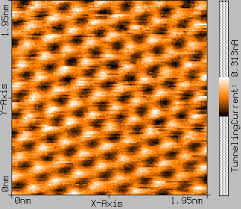
\includegraphics[width=3.4cm]{images.jpeg}};
\end{circuitikz}
}
\caption{Blockschaltbild eines Rastertunnelmikroskops.}

\end{figure}

\end{document}      